\renewcommand{\arraystretch}{1.25}

\subsection*{Applications of the SVD}
\textbf{Principal Component Analysis}

\textit{Principal Component Analysis} (PCA) is a procedure that uses the SVD to analyze data by finding the directions of maximum "spread" or variation. Some of its uses include visualizing high dimensional data and revealing patterns that are useful to perform classification.

Below, we show the steps of performing PCA, as well as visualizations on a two dimensional dataset:

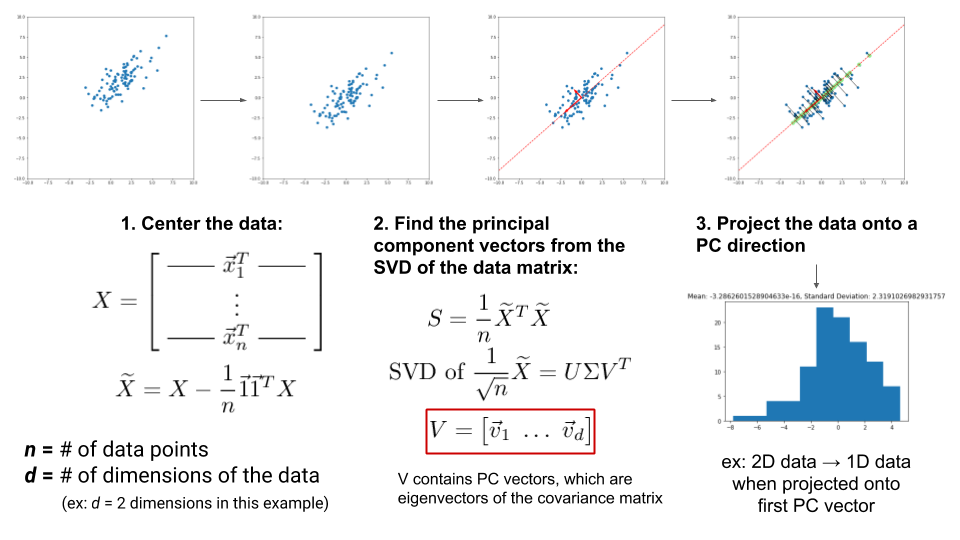
\includegraphics[width=\textwidth]{figures/pca-steps}

\textbf{Minimum Norm Control} \\
\newline
Say we have a controllable system of rank $n$
\begin{align*}
    \vec{x}(k + 1) = A\vec{x}(k) + \vec{b}u(k)
\end{align*}
 and we want to reach a desired state $\vec{x}_f$ with $k > n$ control inputs. We know we can reach any state in $n$ timesteps, and there are infinitely many ways to reach $\vec{x}_f$ in $k > n$ timesteps. Using the SVD, however, we can find the series of control inputs that has the minimum norm.

To solve for the minimum norm solution, we use the \textbf{Moore-Penrose Pseudoinverse}, a generalization of matrix inverses for rectangular matrices using the full SVD of a matrix. We denote the pseudoinverse with a dagger, and the solution will be $\vec{x} = A^{\dagger} \vec{b}.$
This solution is special in that it has \textbf{minimum norm.} That is, if we have another solution $\vec{z},$ such that $A \vec{z} = \vec{b},$ then $\norm{x} \leq \norm{z}.$

To compute the pseudoinverse, we invert each element of the SVD one at a time:

\begin{align*}
    A \vec{x} &= \vec{y} \\
    U \Sigma V^T \vec{x} &= \vec{y} \\
    (U^T U) \Sigma V^T \vec{x} &= U^T \vec{y} \\
    (\Sigma^{\dagger} \Sigma) V^T \vec{x} &= \Sigma^{\dagger} U^T \vec{y} \\
    (V V^T) \vec{x} &= V \Sigma^{\dagger} U^T \vec{y} \\
    \vec{x} &= V \Sigma^{\dagger} U^T \vec{y} \\
    \implies \vec{x} &= A^{\dagger} \vec{y}
\end{align*}

We can calculate $\Sigma^{\dagger}$ accordingly to produce an identity matrix so that the term $\Sigma^{\dagger}\Sigma$ disappears.

$$\Sigma^{\dagger} = \begin{bmatrix} \frac{1}{\sigma_{1}} & 0 &  \cdots & 0 \\ 0 & \frac{1}{\sigma_{2}} & \cdots & 0 \\ \vdots & \vdots & \ddots & \frac{1}{\sigma_{m}} \\ 
    \vdots & \vdots & \ddots & 0 \\ 0 & 0 & 0 & 0 \end{bmatrix}$$

\subsection*{Stability}
A continuous- or discrete-time system is considered \textit{stable} if, for any bounded initial condition and series of inputs, the state remains bounded (if a quantity is \textit{bounded}, it is less than some finite constant at all times). We sometimes refer to this as BIBO (bounded input implies bounded output) stability. \\
\newline
For a system in \textit{discrete time}
$$\vec{x}(k + 1) = A\vec{x}(k) + \vec{b}u(k)$$
The system is
\begin{enumerate}
    \item \textbf{Stable} if all eigenvalues have a \textbf{magnitude less than 1},
    \item \textbf{Unstable} if at least one eigenvalue has a \textbf{magnitude greater than 1}, or
    \item \textbf{Marginally unstable} if at least one eigenvalue has a magnitude of 1 and none have a magnitude greater than 1.
\end{enumerate}

For a system in \textit{continuous time}
$$\frac{d}{dt} \vec{x}(t) = A\vec{x}(t) + \vec{b}u(t)$$
The system is
\begin{enumerate}
    \item \textbf{Stable} if all eigenvalues have a \textbf{negative real component},
    \item \textbf{Unstable} if at least one eigenvalue has a \textbf{positive real component}, or
    \item \textbf{Marginally unstable} if at least one eigenvalue has a real component of 0 and none have a positive real component.
\end{enumerate}

If we plot the eigenvalues on the \textit{complex plane}, a \textbf{discrete-time system} is stable if all eigenvalues are \textbf{strictly inside the unit circle} (left graph), and a \textbf{continuous-time system} is stable if all eigenvalues are on the left half of the plane (right figure): \\
\begin{tabular}{p{0.5\textwidth} p{0.5\textwidth}}
    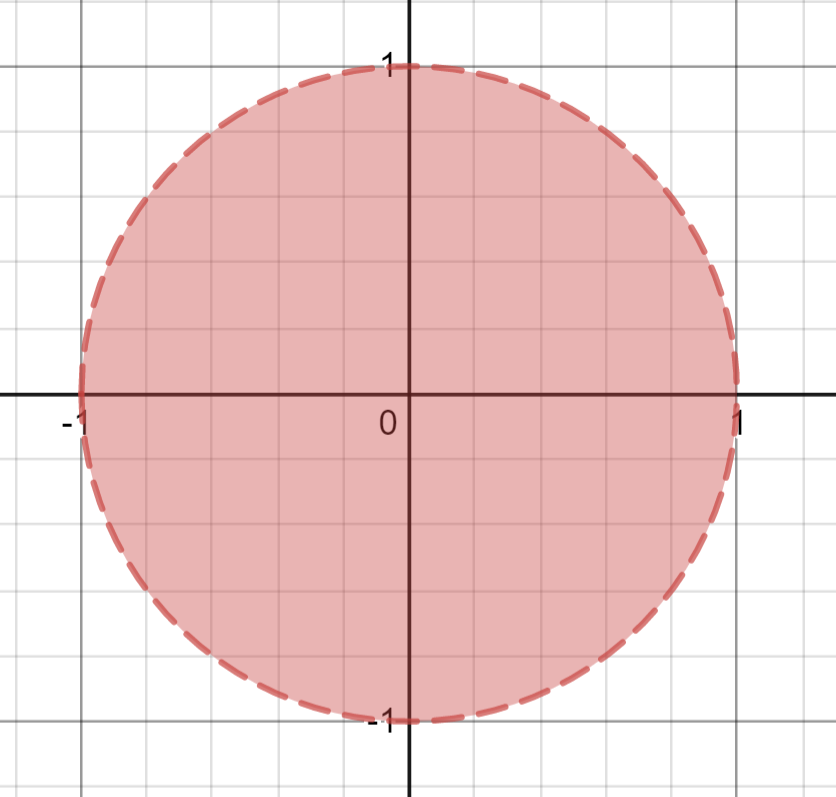
\includegraphics[width = 0.35 \textwidth]{\bank/../sp20/final/figures/discrete-stable.PNG} & 
    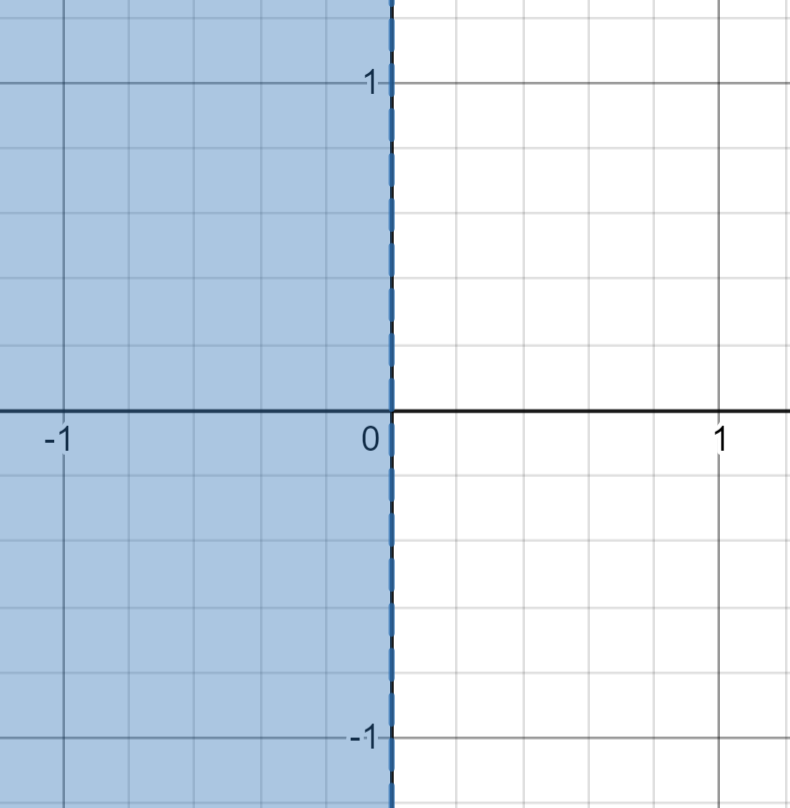
\includegraphics[width = 0.35 \textwidth]{\bank/../sp20/final/figures/continuous-stable.PNG}
\end{tabular}

An interesting case is \textit{upper-triangular matrices}. If a matrix is upper-triangular, its eigenvalues are on the diagonal. So, to see if a system with an upper-triangular A matrix is stable, you can look at the diagonal elements. \\
\newline

\textbf{Visualizing stability}: \\
We know that stable eigenvalues cause any input or initial condition to decay over time, unstable eigenvalues cause the state to grow exponentially, and marginally unstable eigenvalues cause any disturbance to neither decay nor grow. 
In addition, whether or not the eigenvalues have a complex component determines whether the state oscillates (continuous time), or rotates (discrete time). \\
\newline
The following plots will explore how complex eigenvalues affect the state evolution of stable and unstable systems.

\begin{tabular}{|p{0.3\textwidth}| p{0.3\textwidth}|b{0.4\textwidth}|}
    \multicolumn{3}{c}{Plots of $\vec{x}_1(k)$ for discrete-time systems with initial condition $\begin{bmatrix} 1 & 1 \end{bmatrix}^T$} \\
    \hline
    Real and Positive $\lambda$ & Complex or Negative $\lambda$ & Description \\
    \hline & & \\
    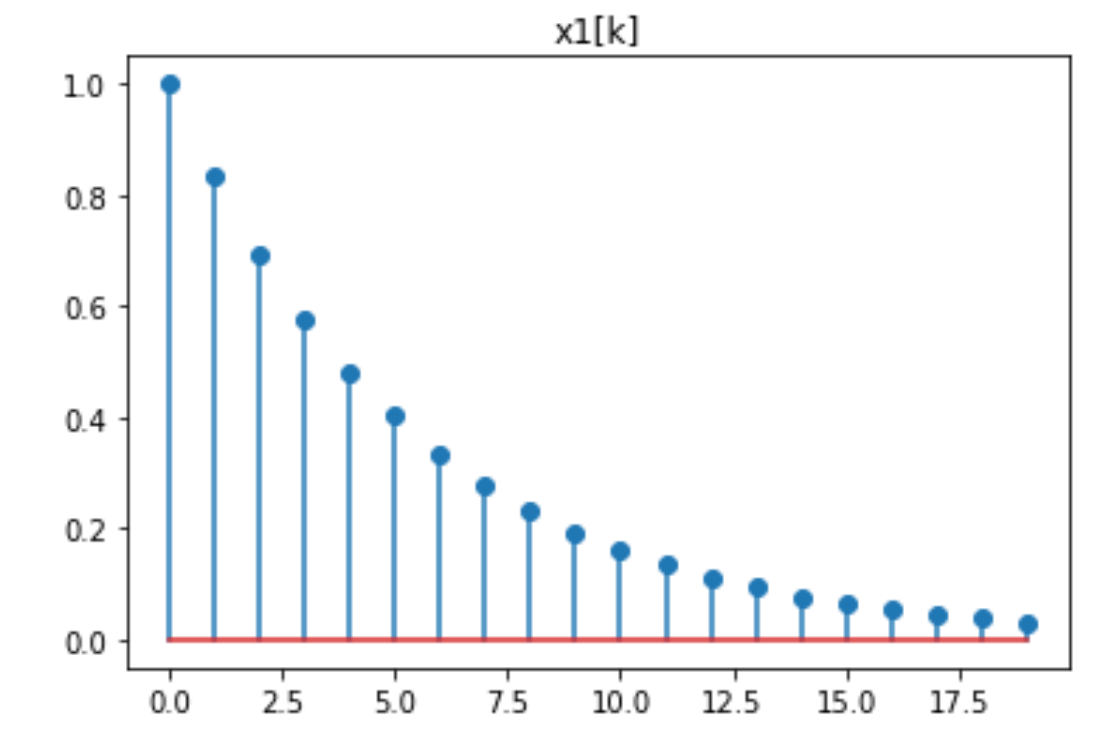
\includegraphics[width = 0.3 \textwidth]{\bank/stability/figures/discrete-graphs/stable-real-x1.PNG} &
    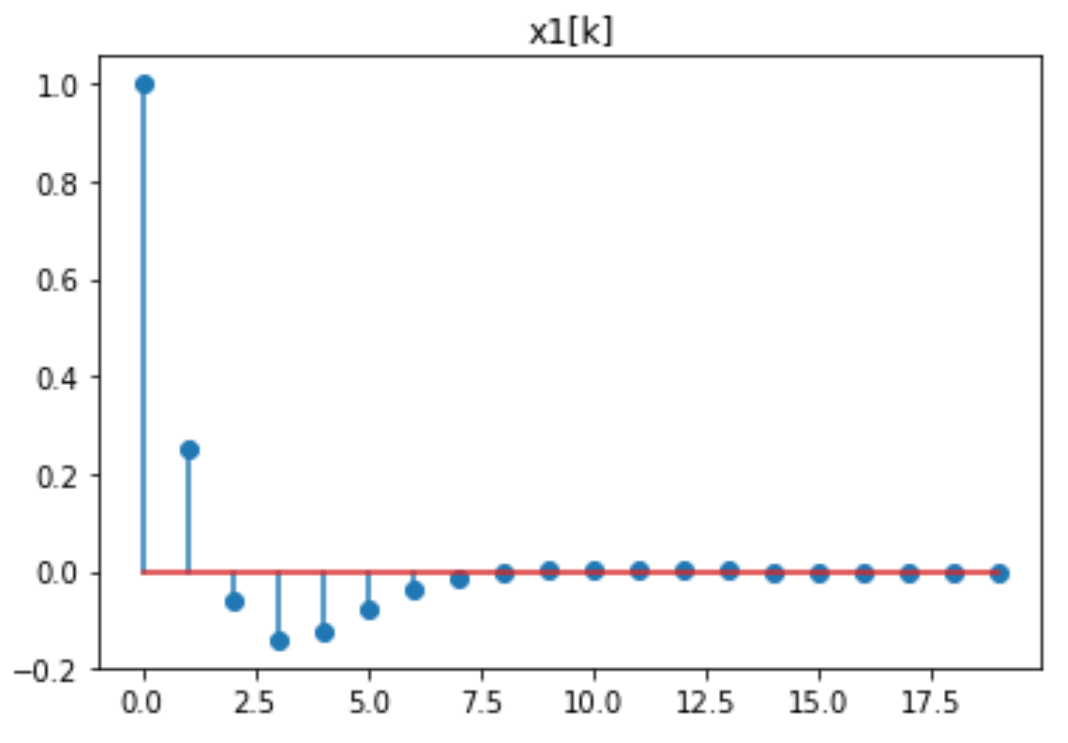
\includegraphics[width = 0.3 \textwidth]{\bank/stability/figures/discrete-graphs/stable-complex-x1.PNG} &
    \textbf{Stable system}: The system is stable, so the initial condition decays over time. When the eigenvalues are \textbf{real}, there is \textbf{no rotation}, but when they are \textbf{complex}, the state vector \textbf{rotates each timestep}. \\
    \hline & & \\
    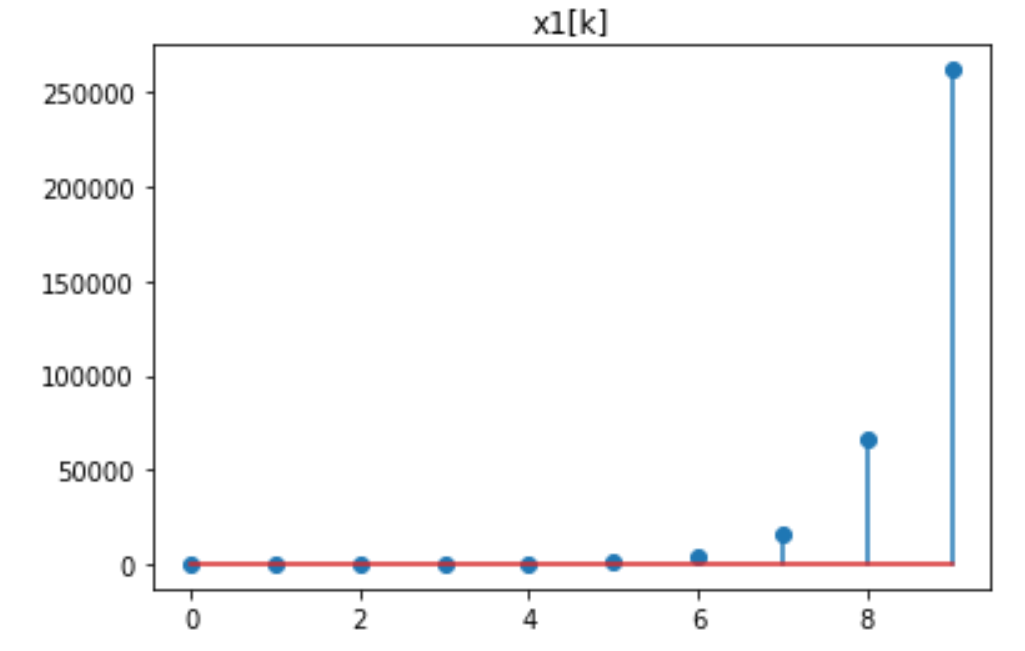
\includegraphics[width = 0.3 \textwidth]{\bank/stability/figures/discrete-graphs/unstable-real-x1.PNG} &
    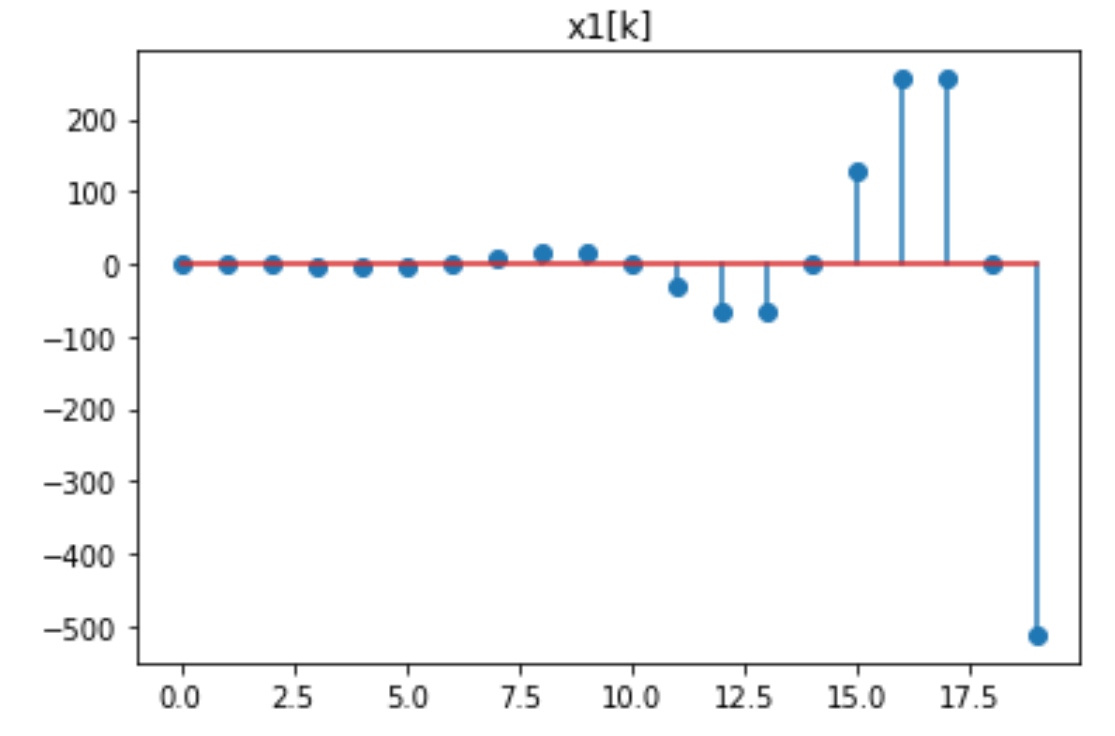
\includegraphics[width = 0.3 \textwidth]{\bank/stability/figures/discrete-graphs/unstable-complex-x1.PNG} &
    \textbf{Unstable system}: The system is unstable, so the initial condition grows exponentially. The state vector rotates only when the eigenvalues are complex. \\
    \hline & & \\
    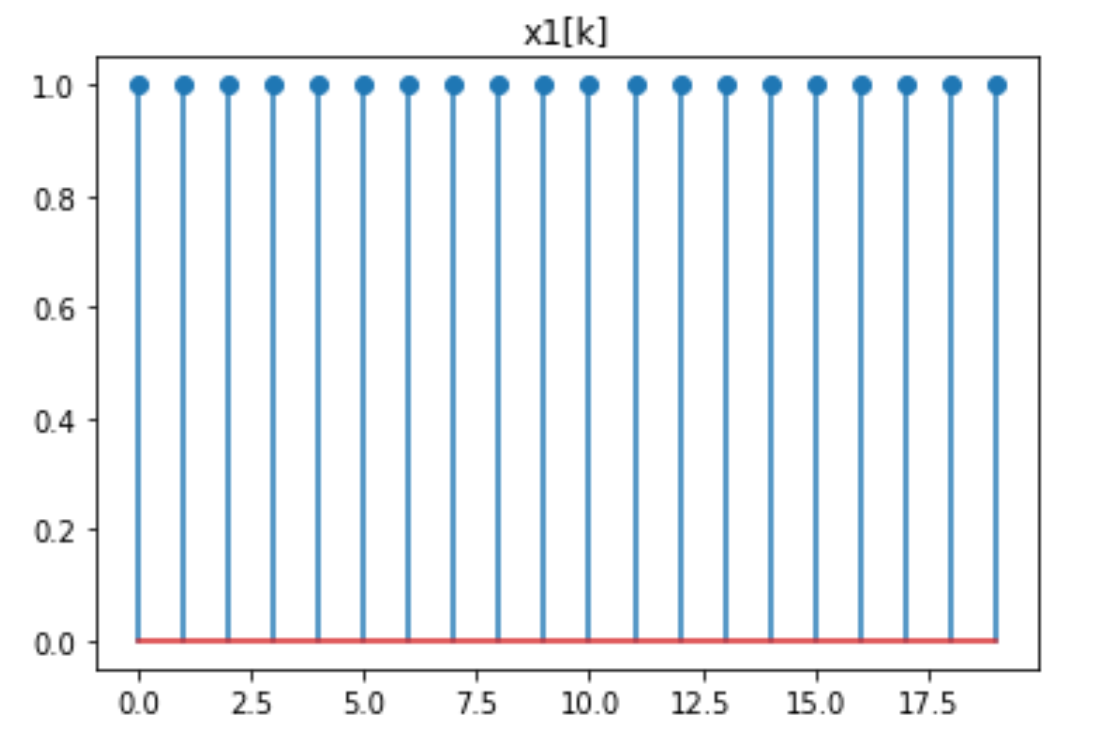
\includegraphics[width = 0.3 \textwidth]{\bank/stability/figures/discrete-graphs/marginal-real-x1.PNG} &
    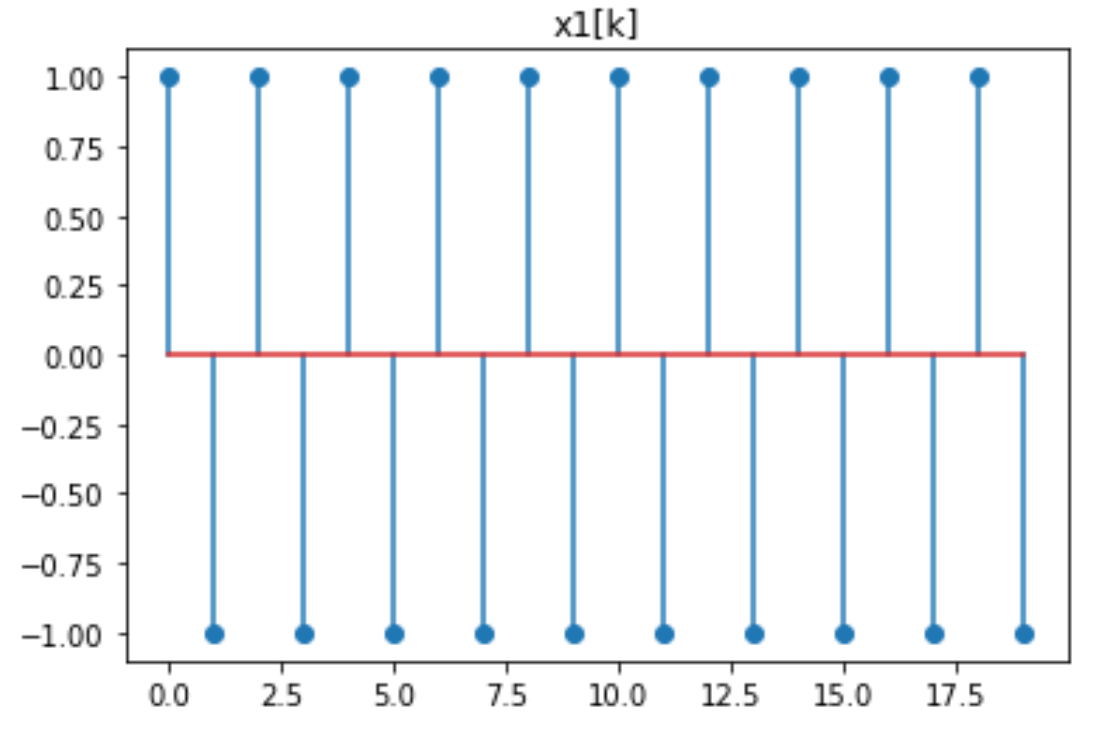
\includegraphics[width = 0.3 \textwidth]{\bank/stability/figures/discrete-graphs/marginal-negative-x1.PNG} &
    \textbf{Marginally unstable}: The initial condition neither grows nor decays. When both eigenvalues are 1, the state vector stays constant. When the eigenvalues are elsewhere on the unit circle, the state vector rotates.\\
    \hline
\end{tabular}

\begin{tabular}{|p{0.3\textwidth}| p{0.3\textwidth}|b{0.4\textwidth}|}
     \multicolumn{3}{c}{Plots of $\vec{x}_1(t)$ for continuous-time systems with initial condition $\begin{bmatrix} 1 & 1 \end{bmatrix}^T$} \\
    \hline
    Real $\lambda$ & Complex or Imag. $\lambda$ & Description \\
    \hline & & \\
    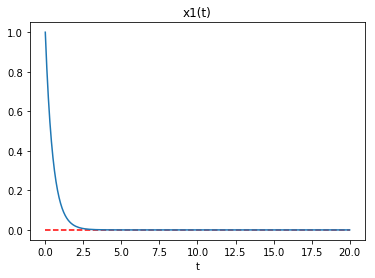
\includegraphics[width = 0.3 \textwidth]{\bank/stability/figures/continuous-graphs/real_negative_x1.png} &
    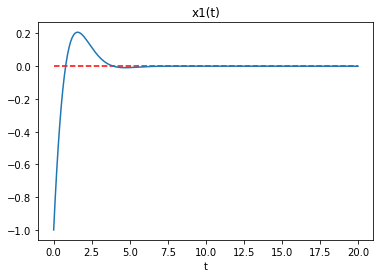
\includegraphics[width = 0.3 \textwidth]{\bank/stability/figures/continuous-graphs/complex_negative_x1.png} &
    \textbf{Stable system}: The system is stable, so the initial condition decays over time. When the eigenvalues are \textbf{real}, there is \textbf{no oscillation}, but when they are \textbf{complex}, the state \textbf{oscillates}. \\
    \hline & & \\
    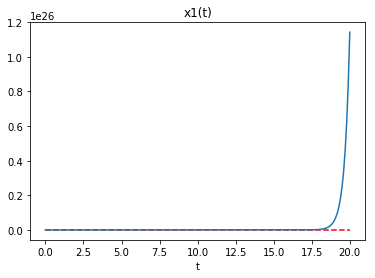
\includegraphics[width = 0.3 \textwidth]{\bank/stability/figures/continuous-graphs/real_positive_x1.png} &
    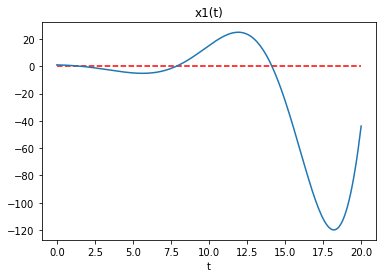
\includegraphics[width = 0.3 \textwidth]{\bank/stability/figures/continuous-graphs/complex_positive_x1.png} &
    \textbf{Unstable system}: The system is unstable, so the initial condition grows exponentially. The state oscillates only when the eigenvalues are complex. \\
    \hline & & \\
    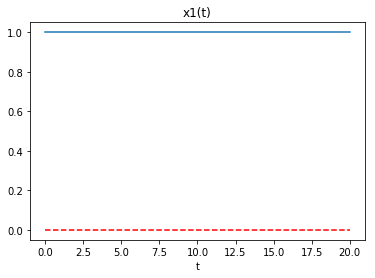
\includegraphics[width = 0.3 \textwidth]{\bank/stability/figures/continuous-graphs/zero_x1.png} &
    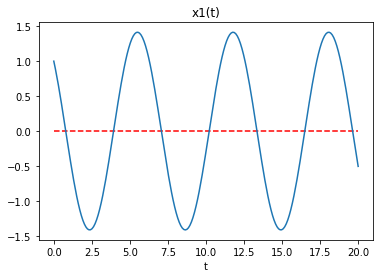
\includegraphics[width = 0.3 \textwidth]{\bank/stability/figures/continuous-graphs/imaginary_x1.png} &
    \textbf{Marginally unstable}: The initial condition neither grows nor decays. When both eigenvalues are 0, the state vector stays constant. When the eigenvalues are imaginary, the state oscillates without decaying.\\
    \hline
\end{tabular}


\subsection*{Feedback Control and Eigenvalue Placement}
Consider a system that is controllable but has unstable eigenvalues:
\begin{align*}
    \vec{x}(k + 1) = A\vec{x}(k) + \vec{b}u(k)
\end{align*}
We can use the fact that the system is controllable to place its eigenvalues wherever we want by applying a \textit{feedback control}, where the control input depends on the current state. Depending on the problem, the feedback input will either be of the form $u(t) = \vec{f^T} \vec{x}(k)$ or $u(t) = -\vec{f^T} \vec{x}(k)$. We will use the first in this worksheet, but you should expect to see both forms.
\begin{align*}
    \vec{x}(k + 1) = A\vec{x}(k) + \vec{b}\vec{f}^T \vec{x}(k)
\end{align*}
We can rewrite this system as follows:
\begin{align*}
    \vec{x}(k + 1) = (A + \vec{b}\vec{f}^T) \vec{x}(k)
\end{align*}
So, the new state transition matrix for the system is $(A + \vec{b}\vec{f}^T)$. Because the system is controllable, we can pick the elements of the feedback coefficient vector $\vec{f}$ to place the eigenvalues of our system wherever we choose. \\
\newline

\textbf{Two-dimensional eigenvalue placement example:}
% TODO Justin

\subsection*{CCF}
It is feasible to calculate feedback control coefficients by hand for a $2 \times 2$ system, but it quickly becomes difficult for higher-order systems. For systems in \textit{controller canonical form (CCF)}, however, it is a lot easier to apply feedback control. \\
\newline
In general, a system in CCF will look like the following:
\begin{align*}
    \vec{x}(k + 1) = \begin{bmatrix}
        0 & 1 & 0 & \cdots & 0 \\
        0 & 0 & 1 & \cdots & 0 \\
        \vdots & \vdots & \vdots & \ddots & \vdots \\
        0 & 0 & 0 & \cdots & 1 \\
        a_1 & a_2 & a_3 & \cdots & a_n
    \end{bmatrix} \vec{x}(k) + \begin{bmatrix}
        0 \\ 0 \\ \vdots \\ 0 \\ 1
    \end{bmatrix} u(k)
\end{align*}
For a system in CCF, the $B$ vector will be \textit{all zeros with a one in the last position}, and $A$ matrix will have \textit{ones in the position to the right of the diagonal and will be zero elsewhere, except in the last row}. \\
\newline
The interesting part about CCF is that the coefficients in the last row of the $A$ matrix \textbf{form the characteristic polynomial of our system}. 
For the above system, the characteristic polynomial would be:
\begin{align*}
    \lambda^n - a_n \lambda^{n - 1} - a_{n - 1}\lambda^{n - 2} - \cdots - a_2 \lambda - a_1 = 0
\end{align*}
Notice that each term after $\lambda^n$ is being \textit{subtracted}, and that the coefficients in the last row of $A$ are ordered in increasing rank (the constant term, then the coefficient of $\lambda$, etc). \\
\newline
Now, let's try to apply a feedback control input to see how useful CCF is.
\begin{align*}
    u(k) = \begin{bmatrix}
        f_1 & \cdots & f_n
        \end{bmatrix} \vec{x} \\
    \vec{x}(k + 1) = \begin{bmatrix}
        0 & 1 & 0 & \cdots & 0 \\
        0 & 0 & 1 & \cdots & 0 \\
        \vdots & \vdots & \vdots & \ddots & \vdots \\
        0 & 0 & 0 & \cdots & 1 \\
        a_1 & a_2 & a_3 & \cdots & a_n
    \end{bmatrix} \vec{x}(k) + \begin{bmatrix}
        0 \\ 0 \\ \vdots \\ 0 \\ 1
    \end{bmatrix} \begin{bmatrix}
        f_1 & \cdots & f_n
        \end{bmatrix} \vec{x}(k)
\end{align*}
The new state transition matrix would be the following:
\begin{align*}
    \begin{bmatrix}
        0 & 1 & 0 & \cdots & 0 \\
        0 & 0 & 1 & \cdots & 0 \\
        \vdots & \vdots & \vdots & \ddots & \vdots \\
        0 & 0 & 0 & \cdots & 1 \\
        a_1 & a_2 & a_3 & \cdots & a_n
    \end{bmatrix} \vec{x}(k) + \begin{bmatrix}
        0 \\ 0 \\ \vdots \\ 0 \\ 1
    \end{bmatrix} \begin{bmatrix}
        f_1 & \cdots & f_n
        \end{bmatrix} = \begin{bmatrix}
        0 & 1 & 0 & \cdots & 0 \\
        0 & 0 & 1 & \cdots & 0 \\
        \vdots & \vdots & \vdots & \ddots & \vdots \\
        0 & 0 & 0 & \cdots & 1 \\
        a_1 + f_1 & a_2 + f_2 & a_3 + f_3 & \cdots & a_n + f_n
    \end{bmatrix}
\end{align*}
And the new characteristic polynomial would be:
\begin{align*}
    \lambda^n - (a_n + f_n)\lambda^{n - 1} - \cdots - (a_2 + f_2) \lambda - (a_1 + f_1)
\end{align*}
As you can see, we can easily set the coefficients of the characteristic polynomial and therefore place the eigenvalues of the system. \\
\newline
% \textbf{CCF transformation and intuition (de-emphasized but in scope)}: \\
% In order to go from an arbitrary \textit{controllable} system to CCF, you can apply the transformation
% $$T = $$